% Copyright 2023 by Johan van der Molen Moris, 2015 by Paul Kirk
%
% This file may be distributed and/or modified
%
% 1. under the LaTeX Project Public License and/or
% 2. under GPLv3.

\documentclass{beamer}
\usetheme[pageofpages=of,% String used between the current page and the total page count.
  ]{BSU}

\usepackage[]{colortbl}
\usepackage{pgf,tikz}
% \usetikzlibrary{positioning,shapes,shadows,arrows}
%  \definecolor{col1}{rgb}{0.2,0.2,0.8}
%  \definecolor{col2}{rgb}{0.5,0.2,0.8}
%  \definecolor{col3}{rgb}{0.8,0.2,0.8}
%  \definecolor{col4}{rgb}{0.2,0.2,0.5}
%  \definecolor{col5}{rgb}{0.2,0.2,0.8}
%  \definecolor{col6}{rgb}{0.8,0.5,0.8}
%  \definecolor{col7}{rgb}{0.8,0.5,0.2}
%  \definecolor{col8}{rgb}{0.8,0.2,0.5}
%  \definecolor{col9}{rgb}{0.5,0.2,0.5}
%  \definecolor{col10}{rgb}{0.5,0.5,0.8}


% \newcommand{\squishlist}{
%  \begin{list}{$\bullet$}
%   { \setlength{\itemsep}{0pt}
%      \setlength{\parsep}{3pt}
%      \setlength{\topsep}{3pt}
%      \setlength{\partopsep}{0pt}
%      \setlength{\leftmargin}{1.5em}
%      \setlength{\labelwidth}{1em}
%      \setlength{\labelsep}{0.5em} } }

% \newcommand{\squishlisttwo}{
%  \begin{list}{$\bullet$}
%   { \setlength{\itemsep}{0pt}
%      \setlength{\parsep}{0pt}
%     \setlength{\topsep}{0pt}
%     \setlength{\partopsep}{0pt}
%     \setlength{\leftmargin}{2em}
%     \setlength{\labelwidth}{1.5em}
%     \setlength{\labelsep}{0.5em} } }

% \newcommand{\squishend}{
%   \end{list}  }

\definecolor{amber}{rgb}{1.0, 0.75, 0.0}
\usepackage{graphicx}
\graphicspath{{./figs/}}
\usepackage{appendixnumberbeamer}

\author[]{Johan van der Molen Moris}
\title[]{Presentation introduction}
\subtitle[]{Presentation introduction subheading}
\institute{MRC Biostatistics Unit}
\date{\today}
%\includeonly{firstpart,secondpart}

%
%Using genomics datasets to identify meaningful subgroups (whether of patients, genes, DNA motifs, or any other biological units) remains a key task in statistical genomics and stratified medicine.  The increasing availability of diverse genomics datatypes presents challenges, as well as opportunities, for subgroup identification.  Here we consider how mixture modelling approaches can be used both for the identification of subgroups and the integration of multiple datatypes.  We also discuss how we can assess (and attempt to maximise) the relevance/meaningfulness of the clusters identified by mixture modelling.
%
%To illustrate, we start by presenting the example of retroviral target integration site identification.  After providing a brief lay summary of the biology, we demonstrate how simple mixture modelling approaches have enabled us to uncover a non-palindromic integration site motif that is shared by multiple retroviruses (including HIV-1 and HTLV-1).
%
%We then present a Bayesian correlated clustering algorithm, which we refer to as MDI (Multiple Dataset Integration). MDI is able to integrate the information from a wide range of different datasets and data types simultaneously (including the ability to model time series data explicitly using Gaussian process regression models). Each dataset is modelled using a Dirichlet-multinomial allocation (DMA) mixture model, with dependencies between these models captured via parameters that describe the levels of agreement among the datasets.  We demonstrate the effectiveness of MDI using a number of examples, including a case study in which we integrate gene expression, ChIP-chip and protein-protein interaction data, to identify a set of protein complexes for which genes are co-regulated during the cell cycle. 
%

\begin{document}
%%%%%%%%%%%%%%%%%%%%%%%%%
%% Title frame 
%%
\begin{frame}[plain]
\titlepage
\setcounter{framenumber}{0}
\end{frame}
%%%%%%%%%%%%%%%%%%%%%%%%%
%

\begin{frame}[t]{Copy Only} 
    % [t] option vertically aligns the text at the top
    % and it makes it look more like the PowerPoint template.
    % When removed the text is centred.
    Quisque sagittis purus sit amet volutpat consequat mauris nunc congue nisi vitae suscipit tellus \textbf{mauris} a diam maecenas sed enim ut sem viverra aliquet eget sit amet tellus cras adipiscing enim eu turpis egestas pretium aenean pharetra magna ac placerat vestibulum lectus mauris ultrices eros in cursus turpis massa tincidunt dui ut ornare lectus sit amet est placerat in egestas erat imperdiet sed euismod nisi porta lorem mollis \textbf{aliquam} ut porttitor leo a diam sollicitudin \textbf{tempor.}
\end{frame}

\begin{frame}[t]{Making your presentations accessible}
  \heading{General guidance}  
  \begin{itemize}
    \item use our primary font Arial for all presentation text
    \item font size should be at least 12-14 point
    \item avoid underlining and italics
    \item use \textbf{bold} for emphasis
    \item avoid writing in all capital letters or all small caps
  \end{itemize}
\end{frame}

\begin{frame}[t]{Making your presentations accessible}
    \heading{Headings}  
    \begin{itemize}
      \item use headings to help people navigate through your content
      \item for headings, use a font size that is at least 20\% larger than the normal text
      \item use \textbf{bold} for emphasis
      \item add extra space around headings and between paragraphs
      \item ensure \alert{\underline{\smash{hyperlinks}}} look different from headings and normal text
    \end{itemize}
  \end{frame}

  \begin{frame}[t]{Making your presentations accessible}
    \heading{Aligning text}  
    \begin{itemize}
      \item left align text, without justification
      \item avoid multiple columns (as used in newspapers)
      \item lines should not be too long: 60 to 70 characters
      \item use white space to group related content
    \end{itemize}
  \end{frame}

  \begin{frame}{Bar chart}
      \begin{minipage}[l]{0.47\textwidth}
        \raggedright
        Quisque sagittis purus sit amet volutpat consequat mauris nunc congue nisi vitae suscipit tellus mauris a diam maecenas sed enim ut sem viverra aliquet eget sit amet tellus cras adipiscing enim eu turpis egestas pretium aenean pharetra magna ac placerat vestibulum lectus mauris ultrices eros in cursus turpis massa tincidunt dui ut ornare lectus.
      \end{minipage}
      \hfill
      \begin{minipage}{0.5\textwidth}
        \centering
        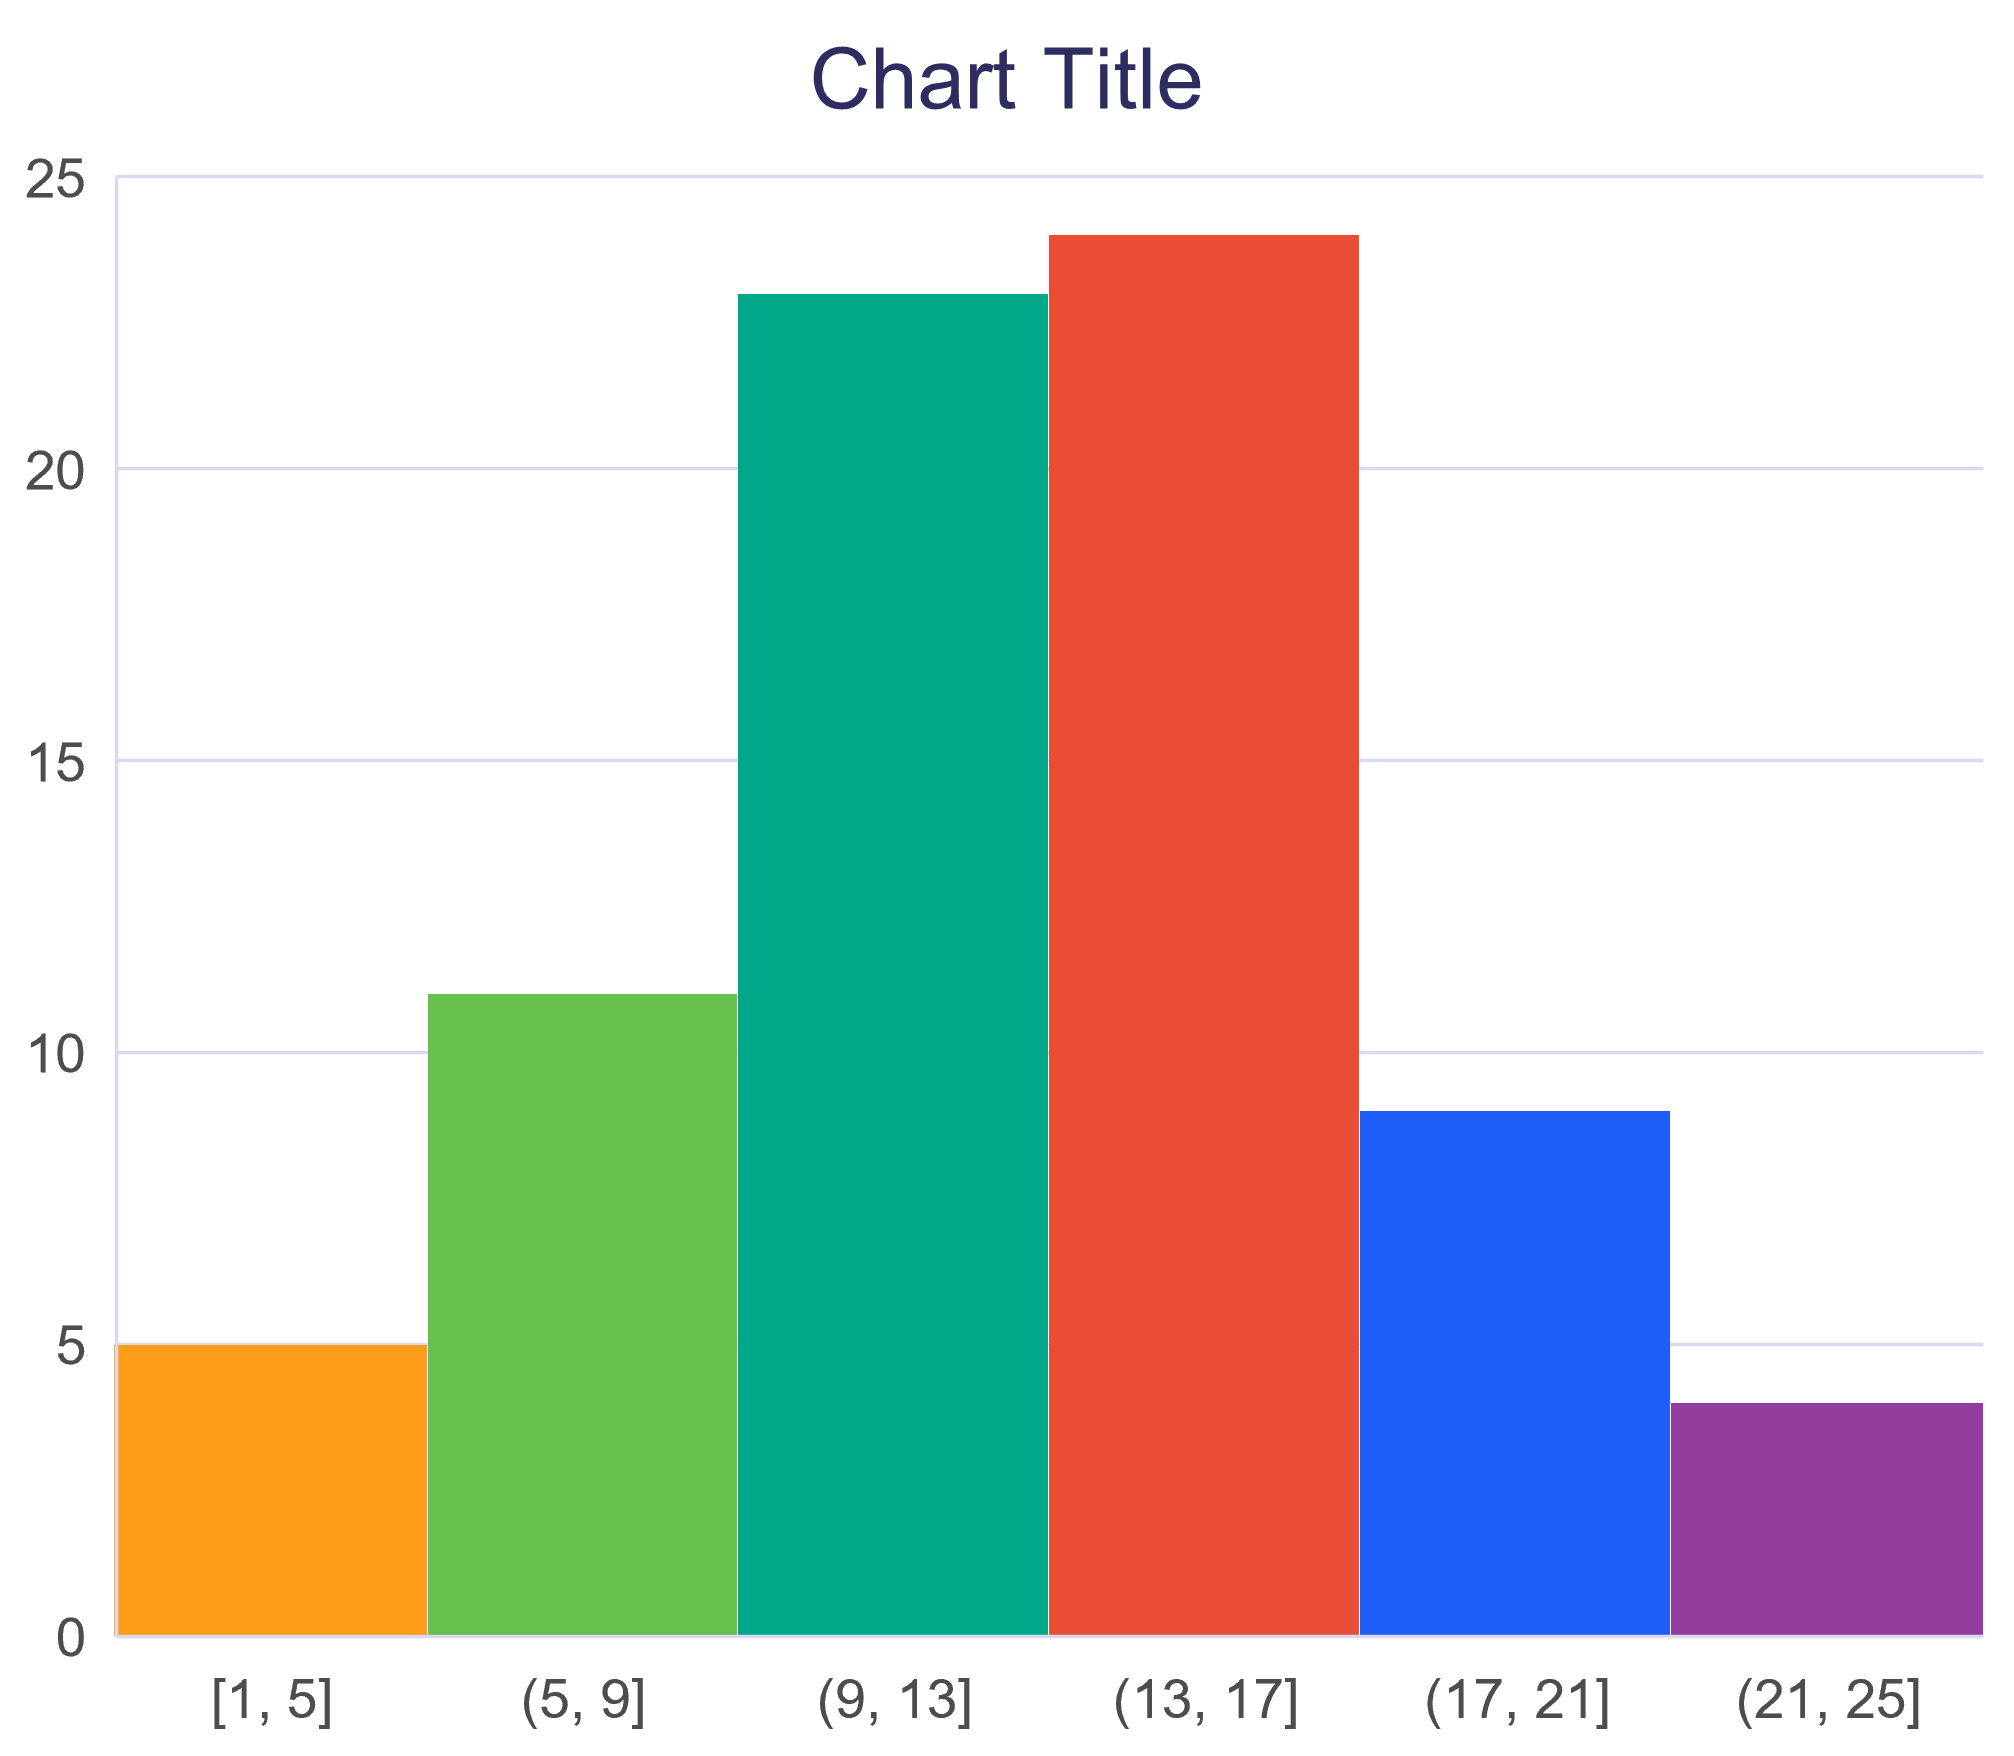
\includegraphics[width=\textwidth]{bar_chart}
      \end{minipage}
  \end{frame}

  \begin{frame}{Blocks}
    \begin{block}{Block}
      Quisque sagittis purus sit amet volutpat consequat mauris      
    \end{block}

    \begin{exampleblock}{Example Block}
      Quisque sagittis purus sit amet volutpat consequat mauris      
    \end{exampleblock}

    \begin{alertblock}{Alerted Block}
      Quisque sagittis purus sit amet volutpat consequat mauris      
    \end{alertblock}
  \end{frame}


  \pgfdeclareimage[width=\paperwidth, height=\paperheight]{BSUbackground2}{background2.png}
  \pgfdeclareimage[width=.65\paperwidth]{BSUpattern2}{pattern2.png}
  \pgfdeclareimage[width=.65\paperwidth]{BSUquestions}{questions.png}
  \begin{frame}[plain]
    \begin{picture}(\paperwidth,\paperheight)
  
        \put(-1in-\oddsidemargin,-1in-\topmargin){%
          \pgfuseimage{BSUbackground2}      
        }
    
        \put(-1in-\oddsidemargin+.03\paperwidth,.81\paperheight){%
          \pgfuseimage{BSUlogo}      
        }

        \put(-1in-\oddsidemargin+.35\paperwidth,0){%
        \pgfuseimage{BSUpattern2}
        }
    
        \put(-1in-\oddsidemargin+.075\paperwidth,.35\paperheight){%
        \pgfuseimage{BSUquestions}
        }

    \end{picture}  
  \end{frame}

  \pgfdeclareimage[width=\paperwidth, height=\paperheight]{BSUbackground3}{background3.png}
  \pgfdeclareimage[width=.65\paperwidth]{BSUthankyou}{thankyou.png}
  \pgfdeclareimage[height=1em]{twitterlogo}{twitterlogo.png}
  \begin{frame}[plain]
    \begin{picture}(\paperwidth,\paperheight)
  
        \put(-1in-\oddsidemargin,-1in-\topmargin){%
          \pgfuseimage{BSUbackground3}      
        }
    
        \put(-1in-\oddsidemargin+.03\paperwidth,.81\paperheight){%
          \pgfuseimage{BSUlogo}      
        }
    
        \put(-1in-\oddsidemargin+.075\paperwidth,.35\paperheight){%
          \pgfuseimage{BSUthankyou}
        }

        \put(-1in-\oddsidemargin+.02\paperwidth,.075\paperheight){%
          {
            \leavevmode%
            \hbox{
              \begin{beamercolorbox}[wd=0.9\paperwidth,ht=.1\paperheight]{footer}
                {MRC Biostatistics Unit \hfil \pgfuseimage{twitterlogo}@MRC\_BSU \hfil mrc-bsu.cam.ac.uk}
              \end{beamercolorbox}
            }
          }
        }

    \end{picture}  
  \end{frame}

\end{document}